\documentclass{article}
\usepackage{tikz, incgraph, hyperref, ocgx, chemfig, hyperref}
\igrset{border=4cm}
\usetikzlibrary{positioning, calc, ocgx, decorations.text, arrows.meta}
\setchemfig{atom sep=20pt, cram width=3pt}
\tikzset{
    default/.append style={
            rectangle,
            rounded corners,
            minimum width=2cm,
            minimum height=1cm
        },
    arrow/.append style={
            -latex,
            shorten >=5pt,
            shorten <=5pt
        },
    line/.append style={
            -,
            shorten >=5pt,
            shorten <=5pt
        },
    deco/.style n args={1}{
            postaction={
                    decorate,
                    decoration={
                            text along path,
                            text align=center,
                            raise=4pt,
                            reverse path,
                            text={#1}
                        }
                }
        }
}
\newcommand{\basic}[2]{
    \begin{ocg}{#1}{#1}{0}
        \textcolor{red}{\hspace{2.5pt}#2}
    \end{ocg}
}
\newcommand{\basicr}[2]{
    \begin{ocg}{#1}{#1}{1}
        \textcolor{red}{\hspace{2pt}#2}
    \end{ocg}
}
\newcommand{\question}[4]{
    \node[default, draw, #1, switch ocg={#2 #2e}](#2){
        \basic{#2}{#3}
    };
    \node at(#2){
        \basicr{#2e}{#4}
    };
}
\newcommand{\questionAt}[4]{
    \node[default, draw, switch ocg={#2 #2e}](#2) at(#1){
        \basic{#2}{#3}
    };
    \node at(#2){
        \basicr{#2e}{#4}
    };
}
\newcommand{\comment}[4]{
    \node[#1,
        switch ocg={#2 #2e}](#2){
        \basic{#2}{#3}
    }
    node[#1]{
        \basicr{#2e}{#4}
    };
}
\newcommand{\commentAt}[4]{
    \node[switch ocg={#2 #2e}](#2) at(#1){
        \basic{#2}{#3}
    }
    node at(#1){
        \basicr{#2e}{#4}
    };
}
\newcommand{\chem}[3]{
    \node[#1](#2){} node at(#2){\setchemfig{cram width=3pt}\chemfig{#3}};
}

\title{Neuroscience}
\date{\today}
\author{unbiased}

\begin{document}
% \maketitle
\begin{inctext}[label={overlay}, overlay={\node at($(page.north)+(0,-3)$){\Huge Transcription};}]
    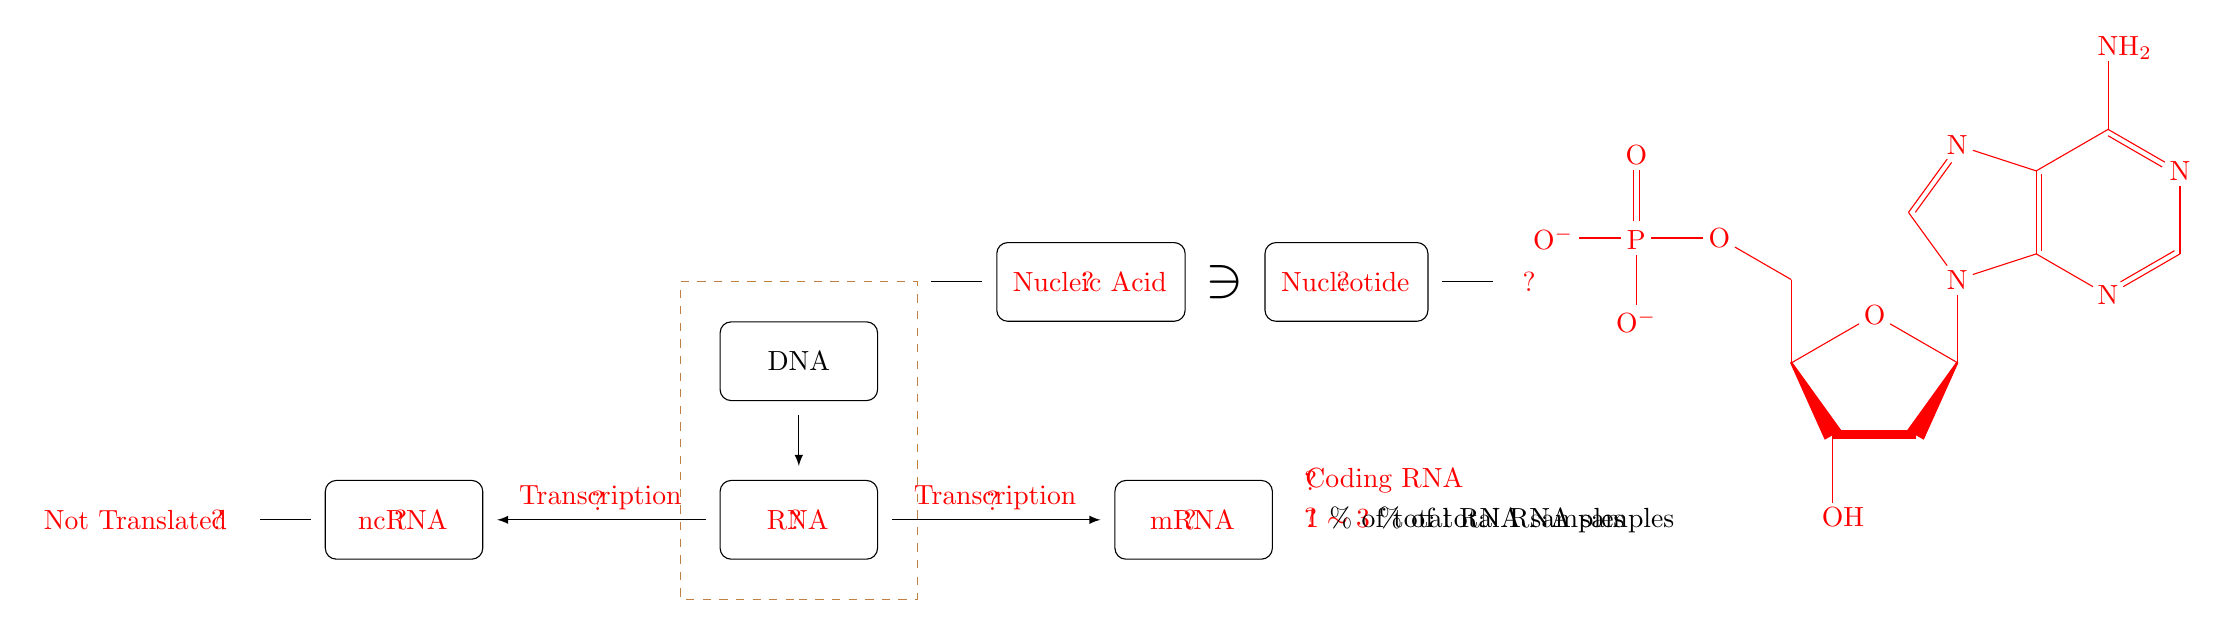
\begin{tikzpicture}
        \node[default, draw](dna){DNA};
\question{below=of dna}{rna}{RNA}{?}
\draw[arrow](dna) to (rna);
\question{right=3cm of rna}{mrna}{mRNA}{?}
\question{left=3cm of rna}{ncRna}{ncRNA}{?}
\draw[arrow](rna) to coordinate(rnaToMrna) (mrna);
\comment{above=0 of rnaToMrna}{transcription}{Transcription}{?}
\draw[arrow](rna) to coordinate(rnaToNcRna) (ncRna);
\comment{above=0 of rnaToNcRna}{ncRnaText}{Transcription}{?}
\comment{right=.2 of mrna}{mrnaText}{$1\sim 3$ \textcolor{black}{\% of total RNA samples}}{? \textcolor{black}{\% of total RNA samples}}
\comment{above=.5 of mrnaText.west, anchor=west}{mrnaTextFirst}{Coding RNA}{?}
\comment{left=of ncRna}{ncRnaTextSecond}{Not Translated}{?}
\draw[line](ncRna) to (ncRnaTextSecond);
\draw[dashed, brown]($(rna.south)+(0,-.5)$)
-| ($(dna.east)+(.5,0)$) |- coordinate(nucleicAcid) ($(dna.north)+(0,.5)$) -| ($(rna.west)+(-.5,0)$) |- cycle;
\question{right=of nucleicAcid}{nucleicAcidText}{Nucleic Acid}{?}
\draw[line](nucleicAcid) to (nucleicAcidText);
\question{right=of nucleicAcidText}{nucleotide}{Nucleotide}{?}
\node at($(nucleicAcidText.east)!.5!(nucleotide.west)$){\huge$\ni$};
\comment{right=of nucleotide}{nucleotideStructure}
{
\chemfig{
O^{-}-P(=[:90]O)(-[:-90]O^{-})-O
-[:-30]-[:-90]([:-18]<[:-60](-[6]OH)-[0,,,,line width=3pt]>[:60]
(-[:90]N
*5([:72]-
*6(-N=-N=(-NH_2)-=)
--N=-))
-[:150,1.15]O-[:210,1.15])
}}{?}
\draw[line](nucleotide) to (nucleotideStructure);

    \end{tikzpicture}
    \chemmove{
        \draw[arrow, blue](hydrogen1) to (oxygen1);
        \commentAt{$(oxygen2)!.5!(hydrogen2)+(-.3,0)$}{fivePrime}{$5^{\prime}$}{?}
        \commentAt{$(oxygen3)!.5!(hydrogen3)+(-.1,.1)$}{threePrime}{$3^{\prime}$}{?}
    }
\end{inctext}
\begin{inctext}[label={overlay}, overlay={\node at($(page.north)+(0,-3)$){\Huge Soma};}]
    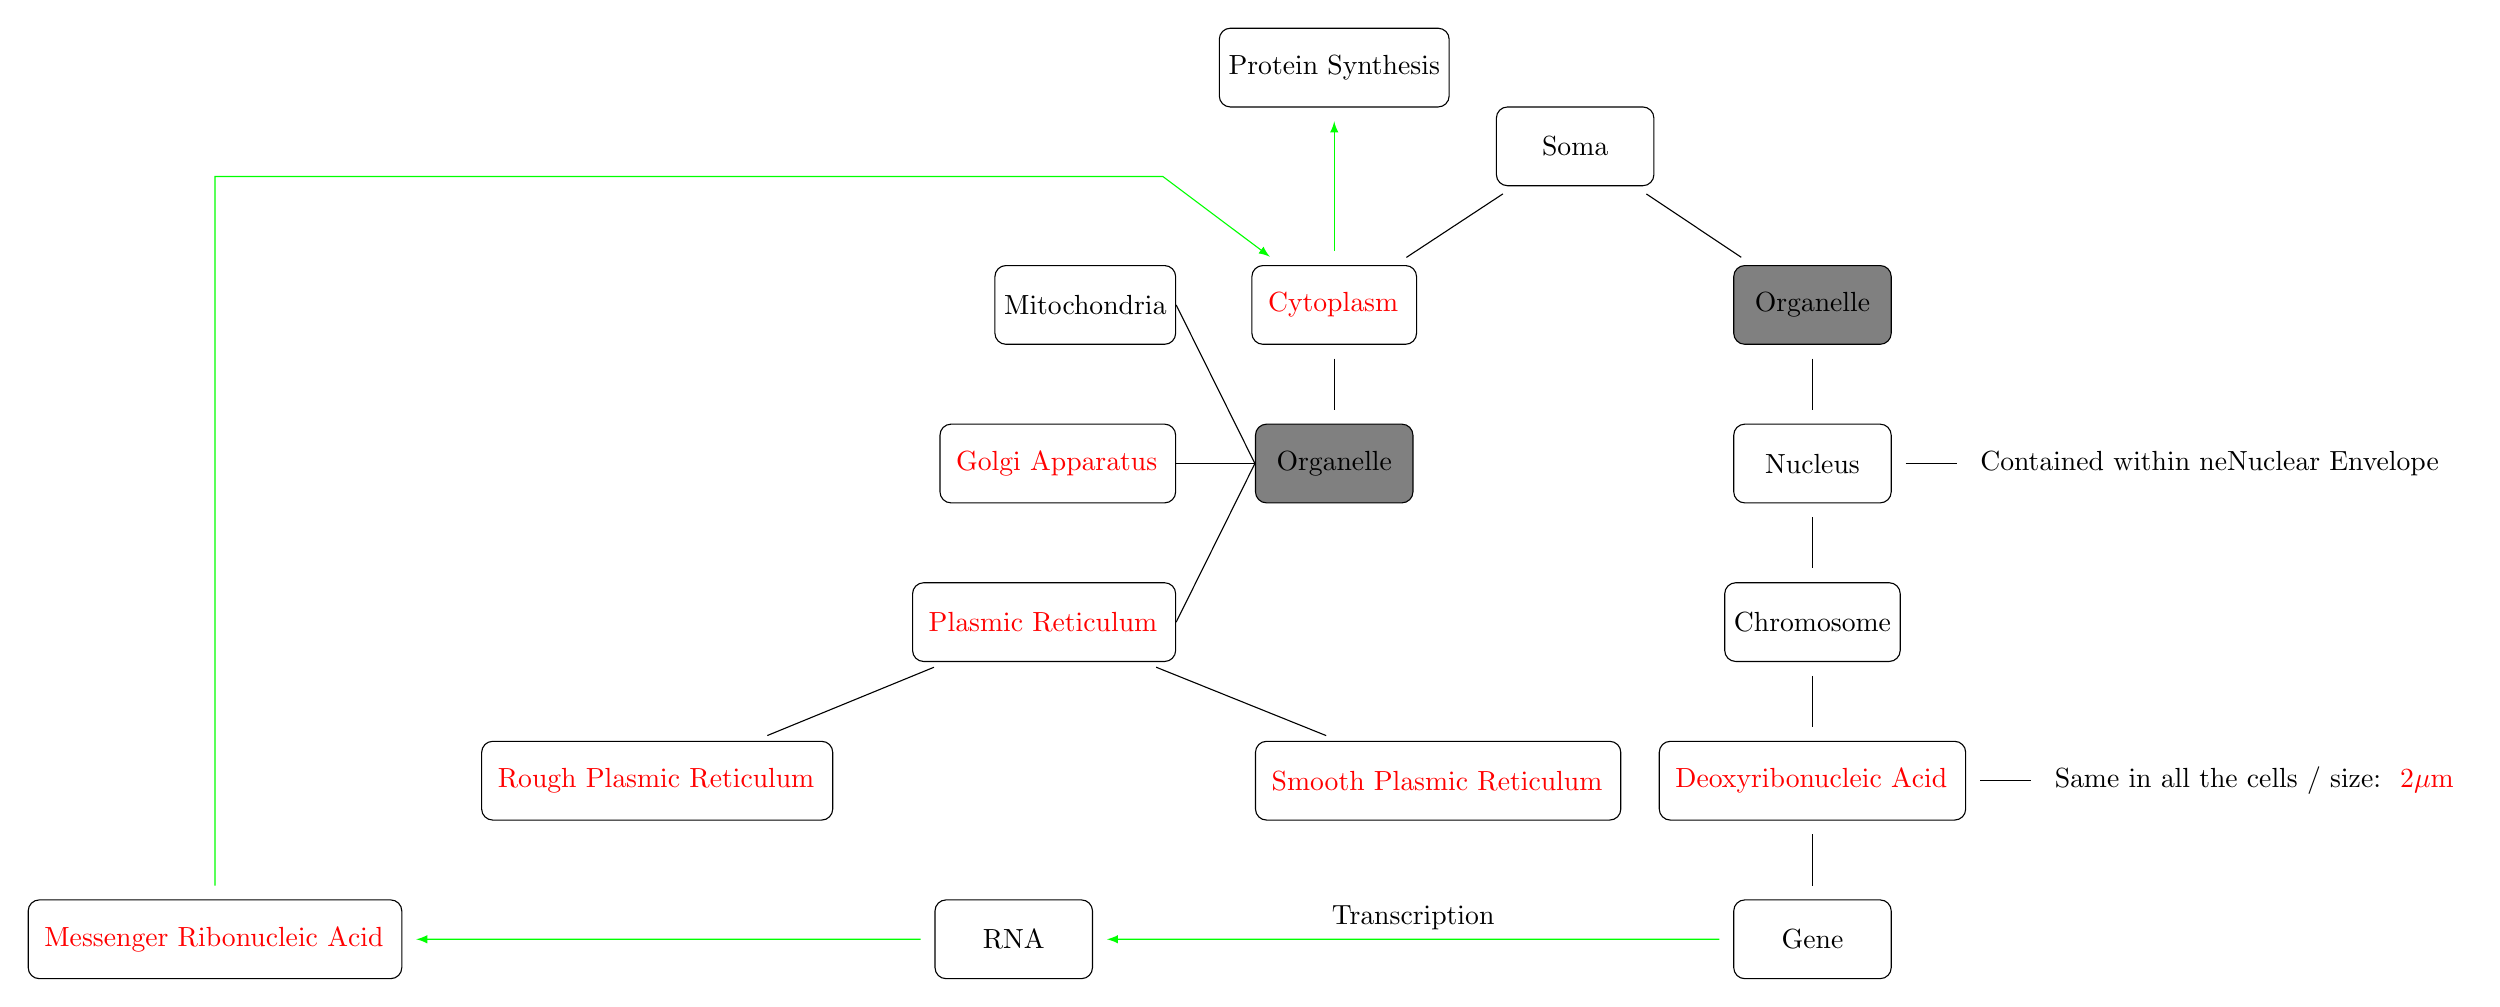
\begin{tikzpicture}
        \node[default, draw](soma){Soma};

\node[default, draw, below left=of soma, switch ocg={cytoplasm}](cytoplasm){
    \basic{cytoplasm}{Cytoplasm}
};
\node[above left=of cytoplasm](space1){};
\node[default, draw, above=2cm of cytoplasm](proteinsynthesis){Protein Synthesis};

\node[default, draw, below right=of soma, fill=gray](organelle2){Organelle};

\node[default, draw, below=of cytoplasm, fill=gray](organelle1){Organelle};
\node[default, draw, below=of organelle2](nucleus){Nucleus};
\node[right=of nucleus, switch ocg={ne}](nuclear envelope){Contained within
    \basicc{ne}{Nuclear Envelope}
};

\node[default, draw, above left=of organelle1](mitochondria){Mitochondria};
\node[default, draw, left=of organelle1, switch ocg={ga}](golgi apparatus){
    \basic{ga}{Golgi Apparatus}
};
\node[default, draw, below left=of organelle1, switch ocg={pr}](plasmic reticulum){
    \basic{pr}{Plasmic Reticulum}
};


\node[default,draw, below left=of plasmic reticulum, switch ocg={rpr}](rough plasmic reticulum){
    \basic{rpr}{Rough Plasmic Reticulum}
};
\node[default, draw, below right=of plasmic reticulum, switch ocg=spr](smooth plasmic reticulum){
    \basic{spr}{Smooth Plasmic Reticulum}
};

\node[default, draw, below=of nucleus](chromosome){Chromosome};
\node[default, draw, below=of chromosome, switch ocg={da}](deoxyribonucleic acid){
    \basic{da}{Deoxyribonucleic Acid}
};
\node[right=of deoxyribonucleic acid, switch ocg={nano}](2nm){
    Same in all the cells / size:\basic{nano}{2$\mu$m}
};
\node[default, draw, below=of deoxyribonucleic acid](gene){Gene};
\node[default, draw, below left=of rough plasmic reticulum, switch ocg={mra}](mrna){
    \basic{mra}{Messenger Ribonucleic Acid}
};
\node[default, draw](rna)at ($(mrna)!.5!(gene)$){RNA};

% ------------------------------------ Arrows -----------------------------------------------------------

\draw[line](soma) to (cytoplasm);
\draw[line](soma) to (organelle2);

\draw[line](organelle2) to (nucleus);

\draw[line](cytoplasm) to (organelle1);

\draw[-](organelle1.west) to (mitochondria.east);
\draw[-](organelle1.west) to (golgi apparatus.east);
\draw[-](organelle1.west) to (plasmic reticulum.east);

\draw[line](plasmic reticulum) to (rough plasmic reticulum);
\draw[line](plasmic reticulum) to (smooth plasmic reticulum);

\draw[line](nucleus) to (chromosome);
\draw[line](nucleus) to (nuclear envelope);

\draw[line](chromosome) to (deoxyribonucleic acid);

\draw[line](deoxyribonucleic acid) to (gene);
\draw[line](deoxyribonucleic acid.east) to (2nm);

\draw[arrow, green](gene) to node[above, black]{Transcription} (rna);
\draw[arrow, green](rna) to (mrna);
\draw[arrow, green](mrna) |- (space1.center) to (cytoplasm);
\draw[arrow, green](cytoplasm) to (proteinsynthesis);
    \end{tikzpicture}
\end{inctext}
\end{document}